
\documentclass[crop,tikz,convert={density=300,size=700x400,outext=.png}]{standalone}

\usepackage{tikz}
\usetikzlibrary{patterns}
\usetikzlibrary{arrows}
\usetikzlibrary{arrows.meta}
\tikzset{>=Triangle}
\usepackage{soul}
\setul{2pt}{.4pt}% 1pt below contents

\newcommand{\componentIcon}[2]{
	% #1: x
	% #2: y
	\draw[fill=white] (#1+.10,#2) rectangle (#1+.4,#2+.4);
	\draw[fill=white] (#1,#2+.08) rectangle (#1+.2,#2+.16);
	\draw[fill=white] (#1,#2+.24) rectangle (#1+.2,#2+.32);
}

\newcommand{\component}[4]{
	% #1: x
	% #2: y
	% #3: name
	% #4: width
	\componentSans{#1}{#2}{#3}{#4};

	\draw (#1+#4/2,#2) to (#1+#4/2,#2-.2);
	\draw[fill=white] (#1+#4/2,#2-.3) circle (.1cm);
}

\newcommand{\componentSans}[4]{
	% #1: x
	% #2: y
	% #3: name
	% #4: width
	\draw[fill=white] (#1,#2) rectangle (#1+#4,#2+1.2);
	\node at (#1+#4/2,#2+.35) {\texttt{#3}};
	\componentIcon{#1+#4-.5}{#2+.7}
}

\begin{document}

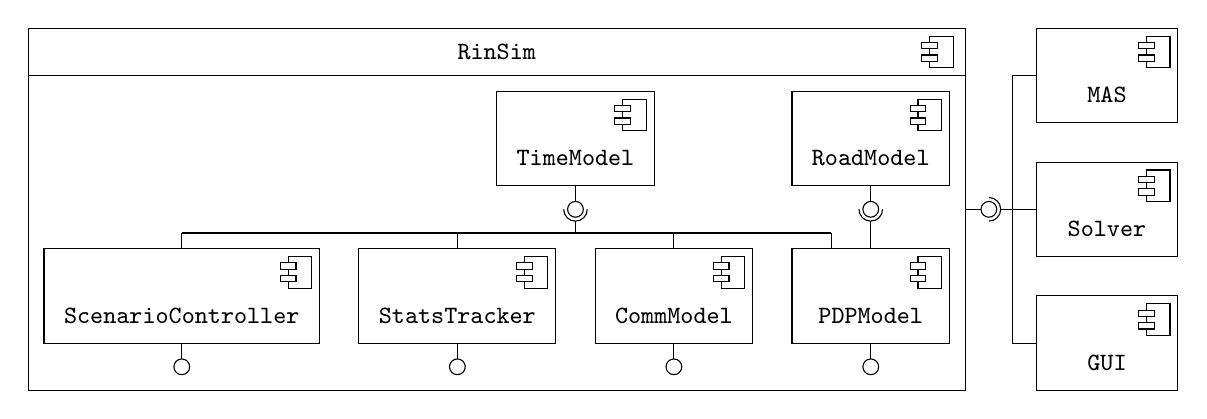
\begin{tikzpicture}[scale=1,every node/.style={font=\small}]

% simulator subsystem
\draw[fill=white] (.8,.4) rectangle (12.7,5.0);
\draw (.8,4.4) to (12.7,4.4);
\node at (6.75,4.7) {\texttt{RinSim}};
\componentIcon{12.15}{4.5}

% TimeModel required interface
\draw (7.6,2.7) arc (180:360:.15cm);
\draw (7.75,2.55) to (7.75,2.4);

% RoadModel required interface
\draw (11.35,2.7) arc (180:360:.15cm);
\draw (11.5,2.55) to (11.5,2.2);

% horizontal
\draw (2.75,2.4) to (11,2.4);

% vertical connect lines
\draw (2.75,2.2) to (2.75,2.4);
\draw (6.25,2.2) to (6.25,2.4);
\draw (9,2.2) to (9,2.4);
\draw (11,2.2) to (11,2.4);

% simulator components
\component{6.75}{3}{TimeModel}{2}
\component{10.5}{3}{RoadModel}{2}
\component{1}{1}{ScenarioController}{3.5}
\component{5}{1}{StatsTracker}{2.5}
\component{8}{1}{CommModel}{2}
\component{10.5}{1}{PDPModel}{2}

% simulator interface
\draw (12.7,2.7) to (12.9,2.7);
\draw[fill=white] (13,2.7) circle (.1cm);
\draw (13,2.55) arc (270:450:.15cm);
\draw (13.15,2.7) to (13.6,2.7);

\draw (13.3,1) to (13.6,1);
\draw (13.3,4.4) to (13.6,4.4);

% vertical
\draw (13.3, 1) to (13.3, 4.4);

% external components
\componentSans{13.6}{3.8}{MAS}{1.8}
\componentSans{13.6}{2.1}{Solver}{1.8}
\componentSans{13.6}{.4}{GUI}{1.8}


\end{tikzpicture}
\end{document}